\newpage
%\thispagestyle {empty}


{\small \listoffigures}
\addcontentsline{toc}{chapter}{Abbildungsverzeichnis} 
\label{Abbildungsverzeichnis}

\begin{figure}[ht]
	\centering
	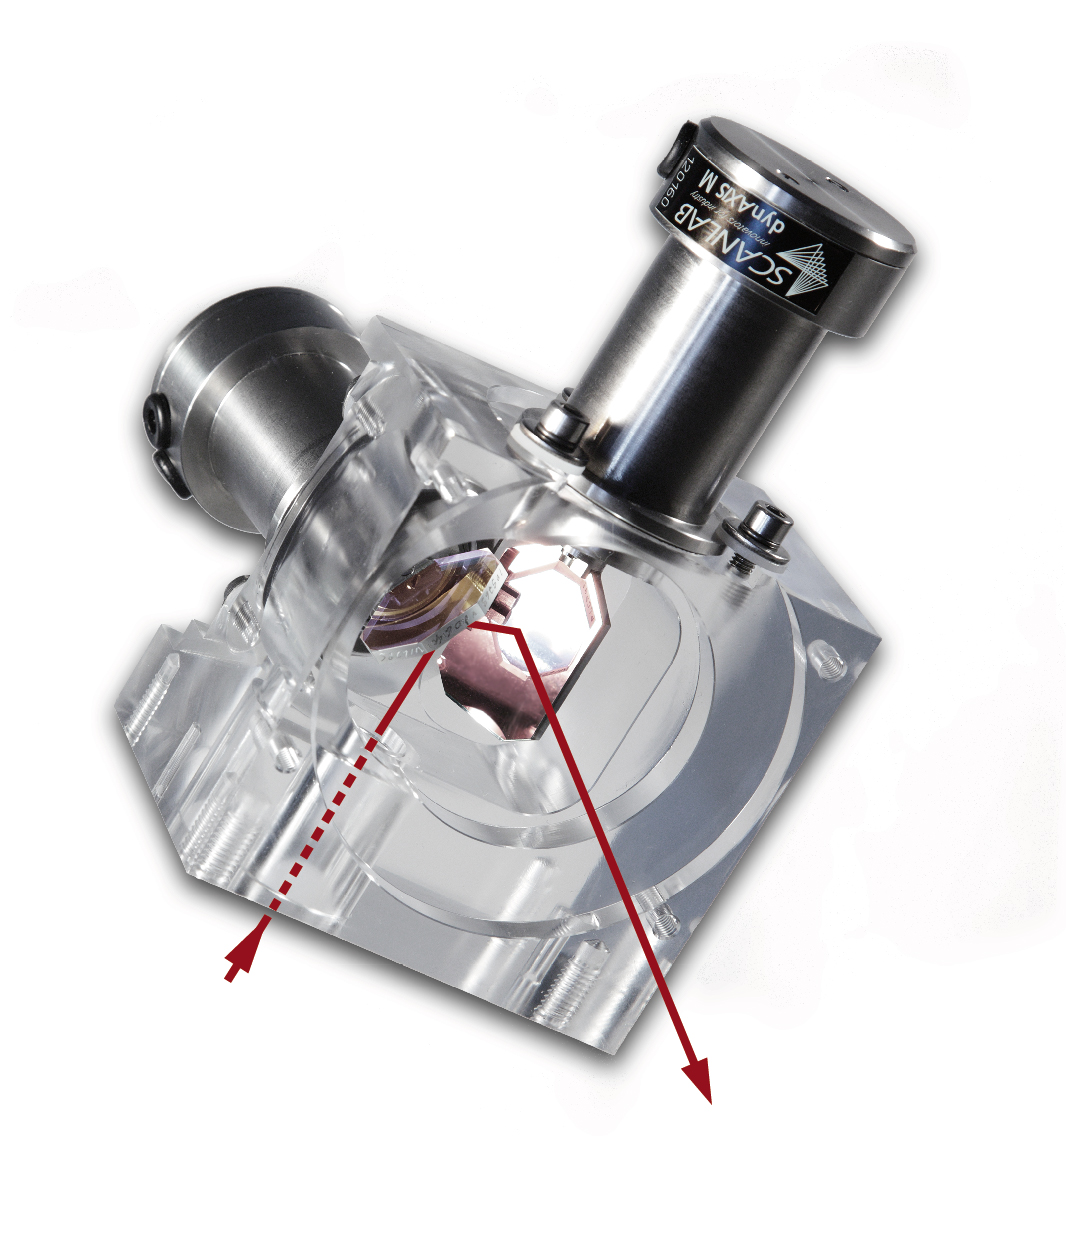
\includegraphics[width=0.6\textwidth]{Plexi_Galvohalter.jpg}
	\caption{2 Laserablenkspiegel\cite{wiki}}
	\label{galvohalter}
\end{figure}
Quelle: http://commons.wikimedia.org/wiki/File:Plexi_Galvohalter.jpg


\begin{figure}[ht]
	\centering
	\includegraphics[width=0.6\textwidth]{Strahlführung.jpg}
	\caption{Fokusebene\cite{lasercommunity}}
	\label{fokusebene}
\end{figure}
Quelle: http://www.laser-community.de/technologie/vw-laser-wobbeln-golf-vii_496/


\begin{figure}[ht]
	\centering
	\includegraphics[width=0.6\textwidth]{Allgemeiner_Aufbau.jpg}
	\caption{Fokusline\cite{selbstgemalt}}
	\label{fokuslinie}
\end{figure}


\begin{figure}[ht]
	\centering
	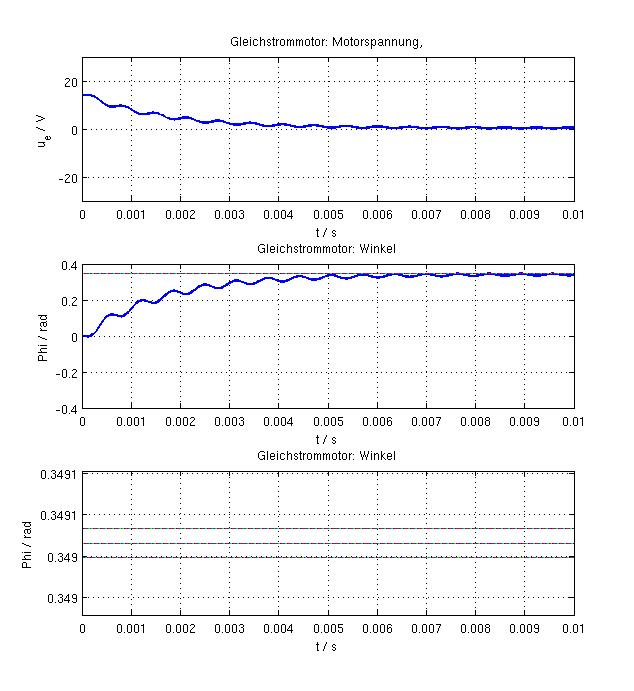
\includegraphics[width=0.6\textwidth]{NurP40.jpg}
	\caption{P-Anteil von 40}
	\label{p40}
\end{figure}


\begin{figure}[ht]
	\centering
	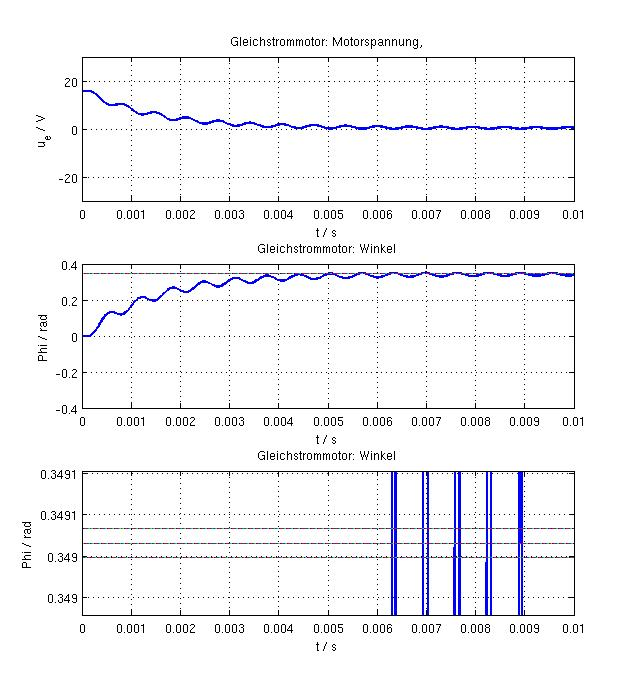
\includegraphics[width=0.6\textwidth]{NurP45.jpg}
	\caption{P-Anteil von 45}
	\label{p45}
\end{figure}


\begin{figure}[ht]
	\centering
	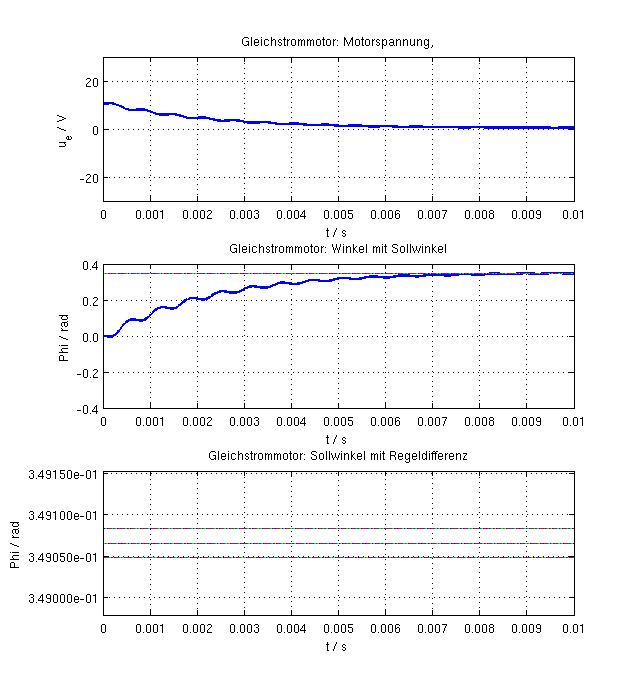
\includegraphics[width=0.6\textwidth]{PI-P30I17.jpg}
	\caption{P-Anteil von 30 und I-Anteil von 17}
	\label{p30i17}
\end{figure}


\begin{figure}[ht]
	\centering
	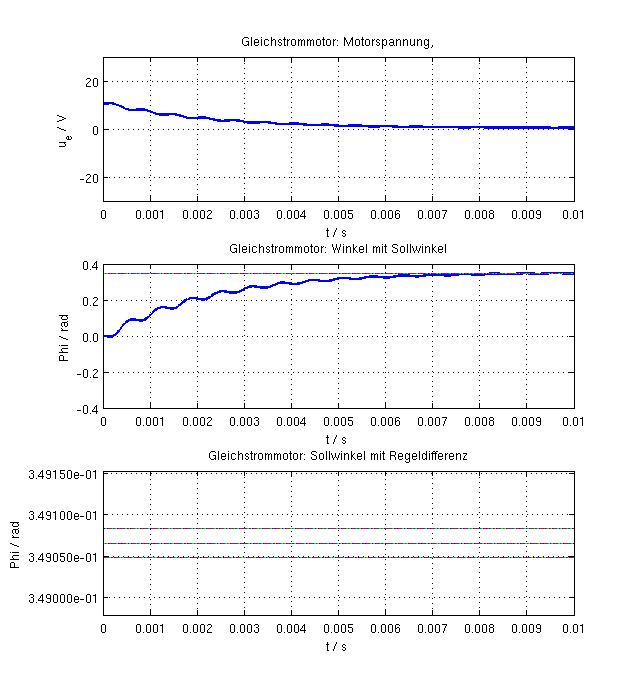
\includegraphics[width=0.6\textwidth]{PI-P30I17.jpg}
	\caption{P-Anteil von 30 und I-Anteil von 17}
	\label{p30i17}
\end{figure}


\begin{figure}[ht]
	\centering
	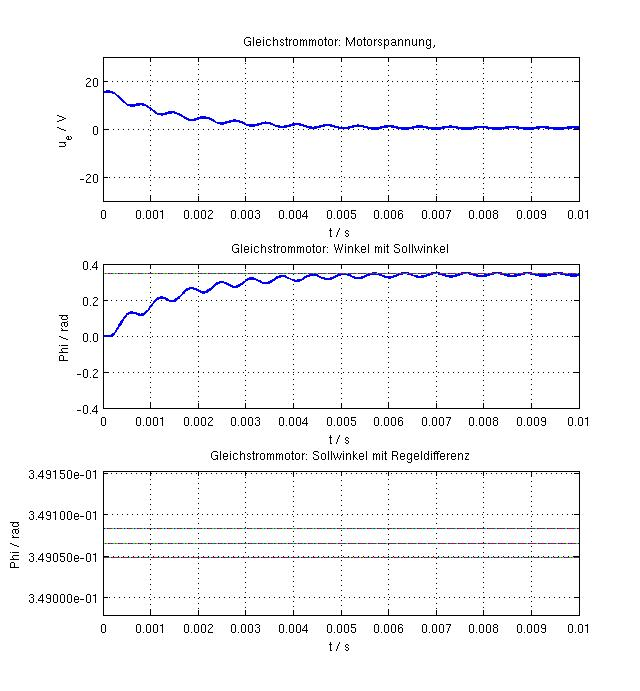
\includegraphics[width=0.6\textwidth]{PD-P22D1N1.jpg}
	\caption{P=22 - D=1 - N=1}
	\label{p22d1n1}
\end{figure}


\begin{figure}[ht]
	\centering
	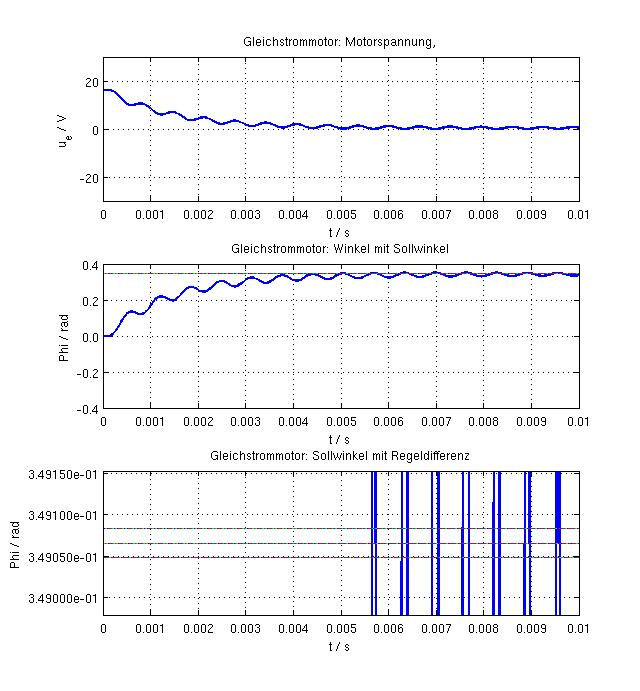
\includegraphics[width=0.6\textwidth]{PD-P23D1N1.jpg}
	\caption{P=22 - D=1 - N=1}
	\label{p23d1n1}
\end{figure}


\begin{figure}[ht]
	\centering
	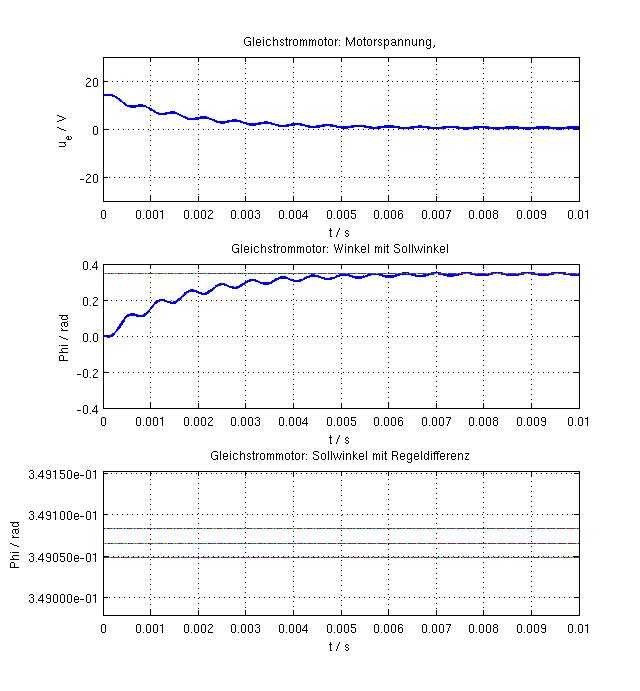
\includegraphics[width=0.6\textwidth]{PID-P20I15D1N1.jpg}
	\caption{P=20 - I=15 - D=1 - N=1}
	\label{p20i15d1n1}
\end{figure}


\begin{figure}[ht]
	\centering
	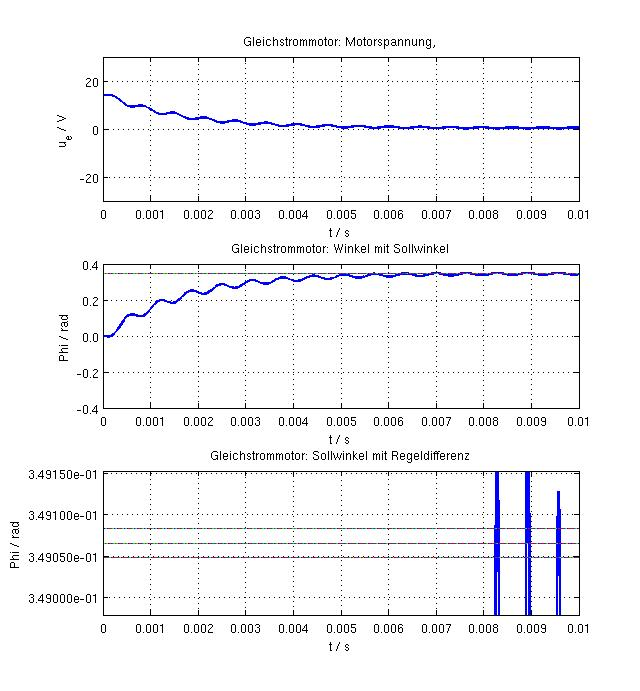
\includegraphics[width=0.6\textwidth]{PID-P20I16D1N1.jpg}
	\caption{P=20 - I=16 - D=1 - N=1}
	\label{p2oi16d1n1}
\end{figure}


\begin{figure}[ht]
	\centering
	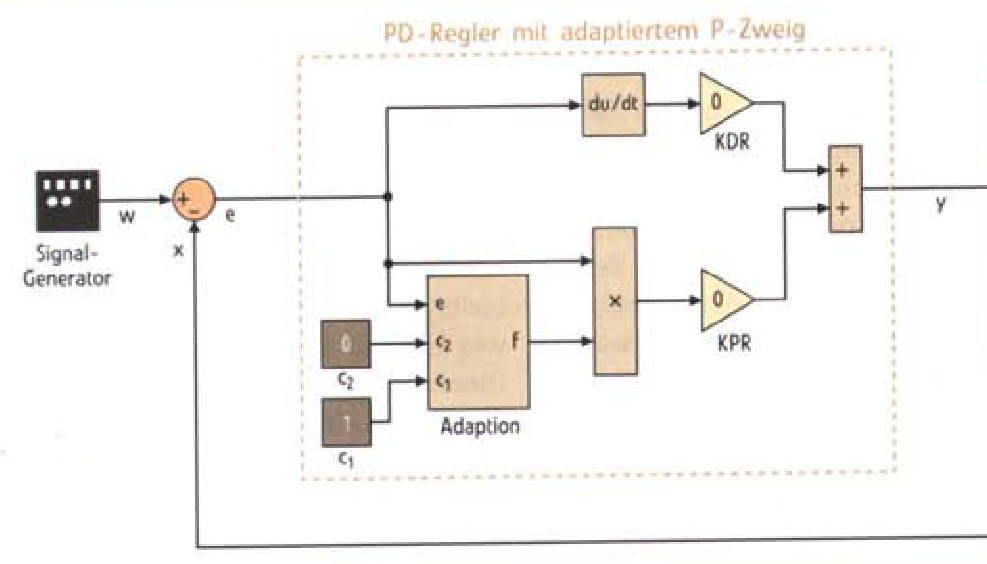
\includegraphics[width=0.6\textwidth]{P-Adaption.jpg}
	\caption{P-Adaption}
	\label{padaption}
\end{figure}


\begin{figure}[ht]
	\centering
	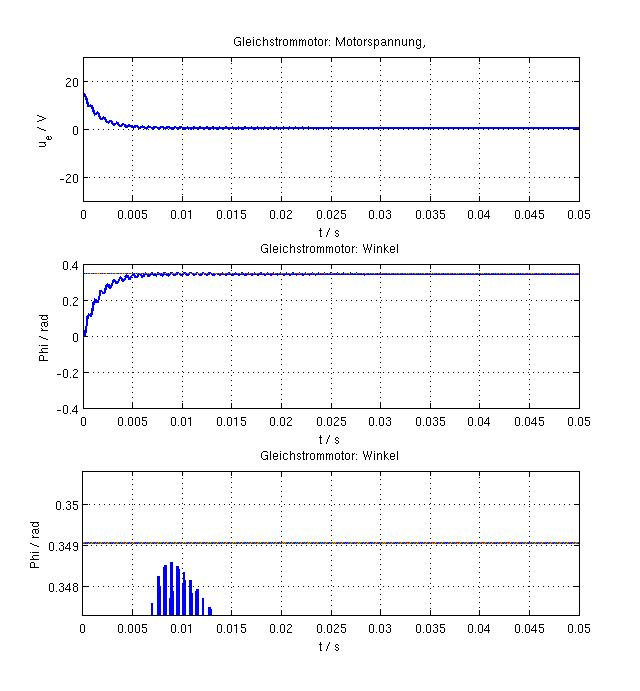
\includegraphics[width=0.6\textwidth]{Pad-P41F1_1,5F2_80.jpg}
	\caption{P-Adaption mit Parametern}
	\label{padp41f1580}
\end{figure}


\begin{figure}[ht]
	\centering
	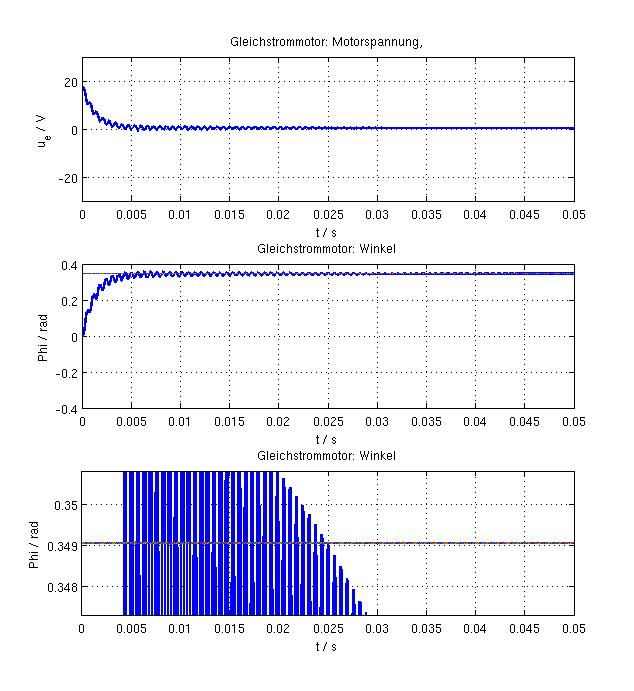
\includegraphics[width=0.6\textwidth]{Pad-P50F1_3F2_400.jpg}
	\caption{P-Adaption mit Parametern}
	\label{padp50f3400}
\end{figure}


\begin{figure}[ht]
	\centering
	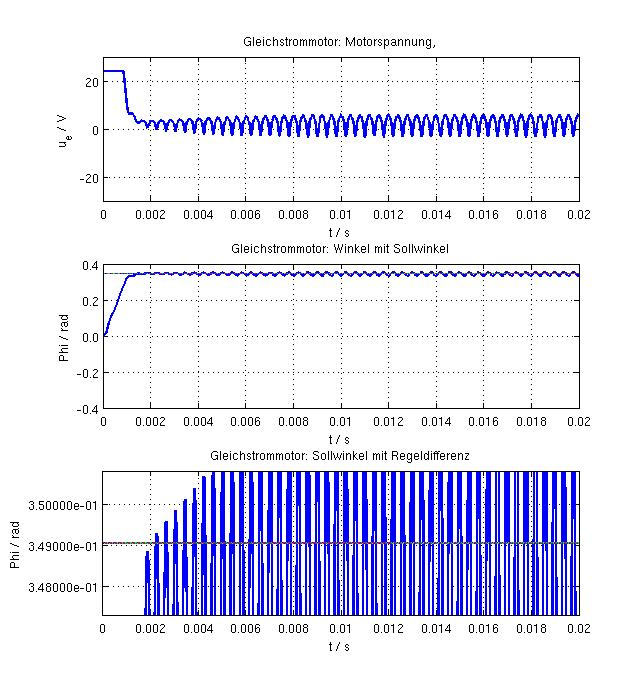
\includegraphics[width=0.6\textwidth]{Pad-Werte-P330F1_5F2_370.jpg}
	\caption{P-Adaption mit neuen Motorparametern}
	\label{padwerte}
\end{figure}


\begin{figure}[ht]
	\centering
	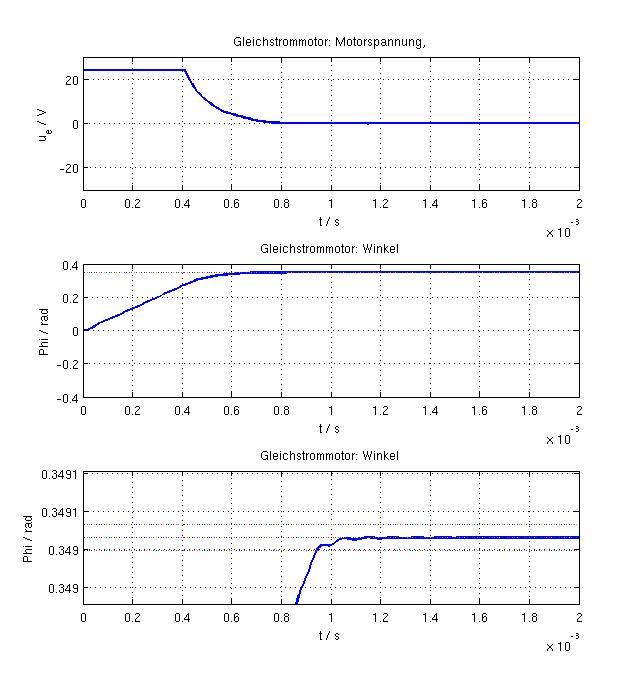
\includegraphics[width=0.6\textwidth]{Pad-Neue-Werte-P320F1_2F2_160.jpg}
	\caption{P-Adaption mit neuen Motorparametern}
	\label{padneuewerte}
\end{figure}
